\chapter{Results} \label{Results}
\label{c4} % la etiqueta para referencias

There are hundreds of possible combinations that can be analyzed by varying the arguments' value and iterations. The main course taken in this chapter is taking essential variations in propagation distance and vortex type and observe how they change as obstructions of larger sizes are imposed over them, and how they compare to the same vortex unobstructed. These results are consistent through changes in state, aperture and number of rings; these results can be further examined in appendix (\ref{Complementary_Results}).

%As it was said in the previous section, the fundamental arguments that generate the phase masks themselves, were not altered to produce the results presented in this section; however, some tests were made varying topological charge and fundamental arguments to test how they affected the outcome. It was decided not include these results here, but in appendix (\ref{Complementary_Results}), for they didn't produce interesting results, in the sense that they didn't provide information that was either new nor useful. On the other hand, variations in staged propagation, distances and obstructions' radii did yield some interesting insights.

As explained in section (\ref{c2:OAM}), the main structure of a vortex consists of a main ring that concentrates most of the beam's intensity, along with a pitch dark central region, consequence of the phase singularity that OAM induces on a beam.

When analyzing the following results, one should be mindful about the inaccuracies that simulations embrace when compared to real life scenarios. For instance, phase masks are not accurate representations, mainly for two reasons: (i) Propagation models introduce errors caused by digital approximations, specifically in the Fourier transforms, integrals and the limited resolution, and (ii) the amount of simultaneous variables that these must handle (refer to figure (\ref{fig:Propagation_Diagram})). In contrast, intensity figures (the OAMs) do represent reality very accurately, meaning that the simulations' results could be easily reproduced in an actual experimental setup.

A final note on how to read the images in this chapter: Most of the images presented here are in \textit{eps} format, meaning that they are vector images. The reader is encouraged to zoom into the images, to unveil more fine details, as no loss of quality will be perceived using a \textit{pdf} reader.

\section{Study of different obstruction radii sizes}
\label{c4: radii size variations}

In this section, $\sigma$, \textit{Rpx} and \textit{N} are fixed at their default values and shown in the title of each figure. Obstructions can deform and compromise the integral ``structure'' of an OAM beam, as described at the beginning of this chapter. Withal, as the obstructions enlarge, these deformations become more prominent, in both cases; however, regular vortices seem to deform more rapidly than perfect ones. 

The aforementioned observations can be examined in figures (\ref{fig:Vortices_r=0_z=1000}) and (\ref{fig:Vortices_r=30_z=1000}); keep in mind that images of perfect vortices (all sub-figures (b) below, bottom-left image titled ``OAM'') are zoomed-in to better visualize them. The first figure shows both regular ((a), left sub-figure) and perfect ((b), right sub-figure) vortices unobstructed (\textit{obstruction\_radius} = 0) and propagated directly through a total distance of 1000 [mm] (\textit{z\_i} = 0 and \textit{z\_f} = 1000). 

Because these vortices are unobstructed, they do not present deformations whatsoever. Their topological charge plot show in figure (\ref{fig:Vortices_r=0_z=1000_TC}) show them both at 10 prominent peaks, representing their topological charge, which is also 10. An examination on their normalized intensity profiles (bottom-right sub-figures, titled ``OAM's Intensity Profile'') confirms this. The two most prominent peaks, that represent the main ring, are practically maxed out, and they form a valley of null intensity, or darkness; this is true for both types.

\begin{figure}[htbp]
    \centering
    \begin{subfigure}[b]{0.45\textwidth}
        \centering
        \includegraphics[width=\textwidth]{images/c04/type=0_r=0_zi=0_zf=1000.eps}
        \caption{Regular vortex.}
    \end{subfigure}
    \hfill
    \begin{subfigure}[b]{0.45\textwidth}
        \centering
        \includegraphics[width=\textwidth]{images/c04/type=1_r=0_zi=0_zf=1000.eps}
        \caption{Perfect vortex.}
    \end{subfigure}
    \caption{Unobstructed vortices directly propagated through $z_f = 1000$ [mm].}
    \label{fig:Vortices_r=0_z=1000}
\end{figure}

\begin{figure}[htbp]
    \centering
    \begin{subfigure}[b]{0.45\textwidth}
        \centering
        \includegraphics[width=\textwidth]{images/c04/type=0_r=0_zi=0_zf=1000_TC.eps}
        \caption{Regular vortex.}
    \end{subfigure}
    \hfill
    \begin{subfigure}[b]{0.45\textwidth}
        \centering
        \includegraphics[width=\textwidth]{images/c04/type=1_r=0_zi=0_zf=1000_TC.eps}
        \caption{Perfect vortex.}
    \end{subfigure}
    \caption{Unobstructed vortices' topological charge.}
    \label{fig:Vortices_r=0_z=1000_TC}
\end{figure}

This is not the case for the obstructed vortices of figure (\ref{fig:Vortices_r=30_z=1000}), where an obstruction of radius 30 [px] was placed upon both type of vortices' phase masks ahead of their respective propagations. As a result, the propagated phase masks (top-right image of each subfigure) and OAMs were deformed. Nonetheless, by once again examining their intensity profiles, the deformations, and lack thereof, are unmistakable. 

In the case of the regular vortex, where its central dark region should be, as seen in the unobstructed scenario, a dim light is found, represented by a small hill in-between the two prominent peaks that are part of the main ring. Additionally, the main ring and its surrounding backlight experienced some sort of deformation, resembling the shape of a camera's shutter. Although the perfect vortex did suffer from loss of intensity in its main ring, slight deformations along its inner edge, and a scritcly non-dark valley, they are not as integral or critical as it was for the regular vortex. 

\begin{figure}[htbp]
    \centering
    \begin{subfigure}[b]{0.45\textwidth}
        \centering
        \includegraphics[width=\textwidth]{images/c04/type=0_r=30_zi=0_zf=1000.eps}
        \caption{Regular vortex.}
    \end{subfigure}
    \hfill
    \begin{subfigure}[b]{0.45\textwidth}
        \centering
        \includegraphics[width=\textwidth]{images/c04/type=1_r=30_zi=0_zf=1000.eps}
        \caption{Perfect vortex.}
    \end{subfigure}
    \caption{Vortices directly propagated through $z_f = 1000$ [mm] with a 30 [px] obstruction radius.}
    \label{fig:Vortices_r=30_z=1000}
\end{figure}

This deformations become more evident for both types as the obstruction size grows to 50 [px] of radius, as shown in figure (\ref{fig:Vortices_r=50_z=1000}). Here, the regular vortex already lost a core property: the region inside the main ring is now brighter than the main ring. As for the perfect one, the region inside the main ring now is covered by a very small, bumpy hill. Despite this, the main ring is still the most intense region and the outer rings have preserved their shapes.

\begin{figure}[htbp]
    \centering
    \begin{subfigure}[b]{0.45\textwidth}
        \centering
        \includegraphics[width=\textwidth]{images/c04/type=0_r=50_zi=0_zf=1000.eps}
        \caption{Regular vortex.}
    \end{subfigure}
    \hfill
    \begin{subfigure}[b]{0.45\textwidth}
        \centering
        \includegraphics[width=\textwidth]{images/c04/type=1_r=50_zi=0_zf=1000.eps}
        \caption{Perfect vortex.}
    \end{subfigure}
    \caption{Vortices directly propagated through $z_f = 1000$ [mm] with a 50 [px] obstruction radius.}
    \label{fig:Vortices_r=50_z=1000}
\end{figure}

\begin{figure}[htbp]
    \centering
    \begin{subfigure}[b]{0.45\textwidth}
        \centering
        \includegraphics[width=\textwidth]{images/c04/type=0_r=50_zi=0_zf=1000_TC.eps}
        \caption{Regular vortex.}
    \end{subfigure}
    \hfill
    \begin{subfigure}[b]{0.45\textwidth}
        \centering
        \includegraphics[width=\textwidth]{images/c04/type=1_r=50_zi=0_zf=1000_TC.eps}
        \caption{Perfect vortex.}
        \label{subfig:Perfect_r=50_z=1000}
    \end{subfigure}
    \caption{Topological charge of vortices propagated through $z_f = 1000$ [mm] with a 50 [px] obstruction radius.}
    \label{fig:Vortices_r=50_z=1000_TC}
\end{figure}

That being said, a quick examination to the topological charge of these obstructed vortices reveals that, apparently, their topological charge has not suffered significant changes.

Finally, with an obstruction of 100 [px] of radius (figure (\ref{fig:Vortices_r=100_z=1000})), the regular vortex essentially becomes a Gaussian beam surrounded by petal-like spotlights. Now the perfect one's central region is now uniformly lit; nonetheless, the main ring still is the most intense region. Do notice that the outer rings have now deformed as much as the central ring. Even though the main structure visually appears to be there, the intensity profile alerts that the center might be giving out a critical compromise.

\begin{figure}[htbp]
    \centering
    \begin{subfigure}[b]{0.45\textwidth}
        \centering
        \includegraphics[width=\textwidth]{images/c04/type=0_r=100_zi=0_zf=1000.eps}
        \caption{Regular vortex.}
    \end{subfigure}
    \hfill
    \begin{subfigure}[b]{0.45\textwidth}
        \centering
        \includegraphics[width=\textwidth]{images/c04/type=1_r=100_zi=0_zf=1000.eps}
        \caption{Perfect vortex.}
    \end{subfigure}
    \caption{Vortices directly propagated through $z_f = 1000$ [mm] with a 100 [px] obstruction radius.}
    \label{fig:Vortices_r=100_z=1000}
\end{figure}

\begin{figure}[htbp]
    \centering
    \begin{subfigure}[b]{0.45\textwidth}
        \centering
        \includegraphics[width=\textwidth]{images/c04/type=0_r=100_zi=0_zf=1000_TC.eps}
        \caption{Regular vortex.}
    \end{subfigure}
    \hfill
    \begin{subfigure}[b]{0.45\textwidth}
        \centering
        \includegraphics[width=\textwidth]{images/c04/type=1_r=100_zi=0_zf=1000_TC.eps}
        \caption{Perfect vortex.}
    \end{subfigure}
    \caption{Topological charge of vortices propagated through $z_f = 1000$ [mm] with a 100 [px] obstruction radius.}
    \label{fig:Vortices_r=100_z=1000_TC}
\end{figure}

On the side of the topological charge, once again, it does not show relevant changes. Although one might notice that the perfect vortex's plot has curvier ramps, it does not affect the number of peaks, which holds at 10, as it is expected. This helps us to conclude that, even though the obstruction size does significantly affect the shape and structure of the OAM in intensity, it does seem to reflect such drastic shifts in its phase, at least not enough to alter the topological charge.

In summary, this set of results show that regular vortices are more susceptible to deformation when coming across a central circular obstruction, in comparison to perfect vortices.

\section{Study of different propagation distances}
\label{c4:z_f variations}

Following the same logic line, this section studies the outcomes of changing the final propagation distance, mainly. Regardless, a similar evolution for $z_f = \infty$ will be presented as well. 

At 1500 [mm] and an obstruction of 50 [px] of radius, both vortices show an enhanced resistance to the deformities that the obstructions present, compared with $z_f = 1000$ [mm] (figure (\ref{subfig:Perfect_r=50_z=1000})); yet, the regular vortices still break down faster than the perfect ones. This comparison is illustrated directly in figure (\ref{fig:perfects_1000_vs_1500}).

\begin{figure}[htbp]
    \centering
    \begin{subfigure}[b]{0.45\textwidth}
        \centering
        \includegraphics[width=\textwidth]{images/c04/type=0_r=50_zi=0_zf=1500.eps}
        \caption{Regular vortex.}
    \end{subfigure}
    \hfill
    \begin{subfigure}[b]{0.45\textwidth}
        \centering
        \includegraphics[width=\textwidth]{images/c04/type=1_r=50_zi=0_zf=1500.eps}
        \caption{Perfect vortex.}
    \end{subfigure}
    \caption{Vortices directly propagated through $z_f = 1500$ [mm] with a 50 [px] obstruction radius.}
    \label{fig:Vortices_r=50_z=1500}
\end{figure}

\begin{figure}[htbp]
    \centering
    \begin{subfigure}[b]{0.45\textwidth}
        \centering
        \includegraphics[width=\textwidth]{images/c04/type=0_r=50_zi=0_zf=1500_TC.eps}
        \caption{Regular vortex.}
    \end{subfigure}
    \hfill
    \begin{subfigure}[b]{0.45\textwidth}
        \centering
        \includegraphics[width=\textwidth]{images/c04/type=1_r=50_zi=0_zf=1500_TC.eps}
        \caption{Perfect vortex.}
    \end{subfigure}
    \caption{Topological charge of vortices propagated through $z_f = 1500$ [mm] with a 50 [px] obstruction radius.}
    \label{fig:Vortices_r=50_z=1500_TC}
\end{figure}

As for the topological charge, we acquire more evidence implying that neither distance nor obstruction size seem to affect the effective topological charge that the phase mask shows. It is noteworthy that the ramps in the perfect vortex's plot are more erratic than at $z_f = 1000$ [mm].

Comparing the intensity profile of a perfect vortex with a 50 [px] obstruction radius propagated at 1000 [mm] and 1500 [mm] (figure (\ref{fig:perfects_1000_vs_1500})) shows that increasing $z_f$ helps to enhance its resistance. The main ring remained brighter by the end of the longer propagation, and the hill between the peaks in significantly smaller. In general, the results suggest that larger the propagation distances increase vortex resistance to deformation, as long as an unobstructed mask can also produce a vortex at the same propagation distance. 

\begin{figure}[htbp]
    \centering
    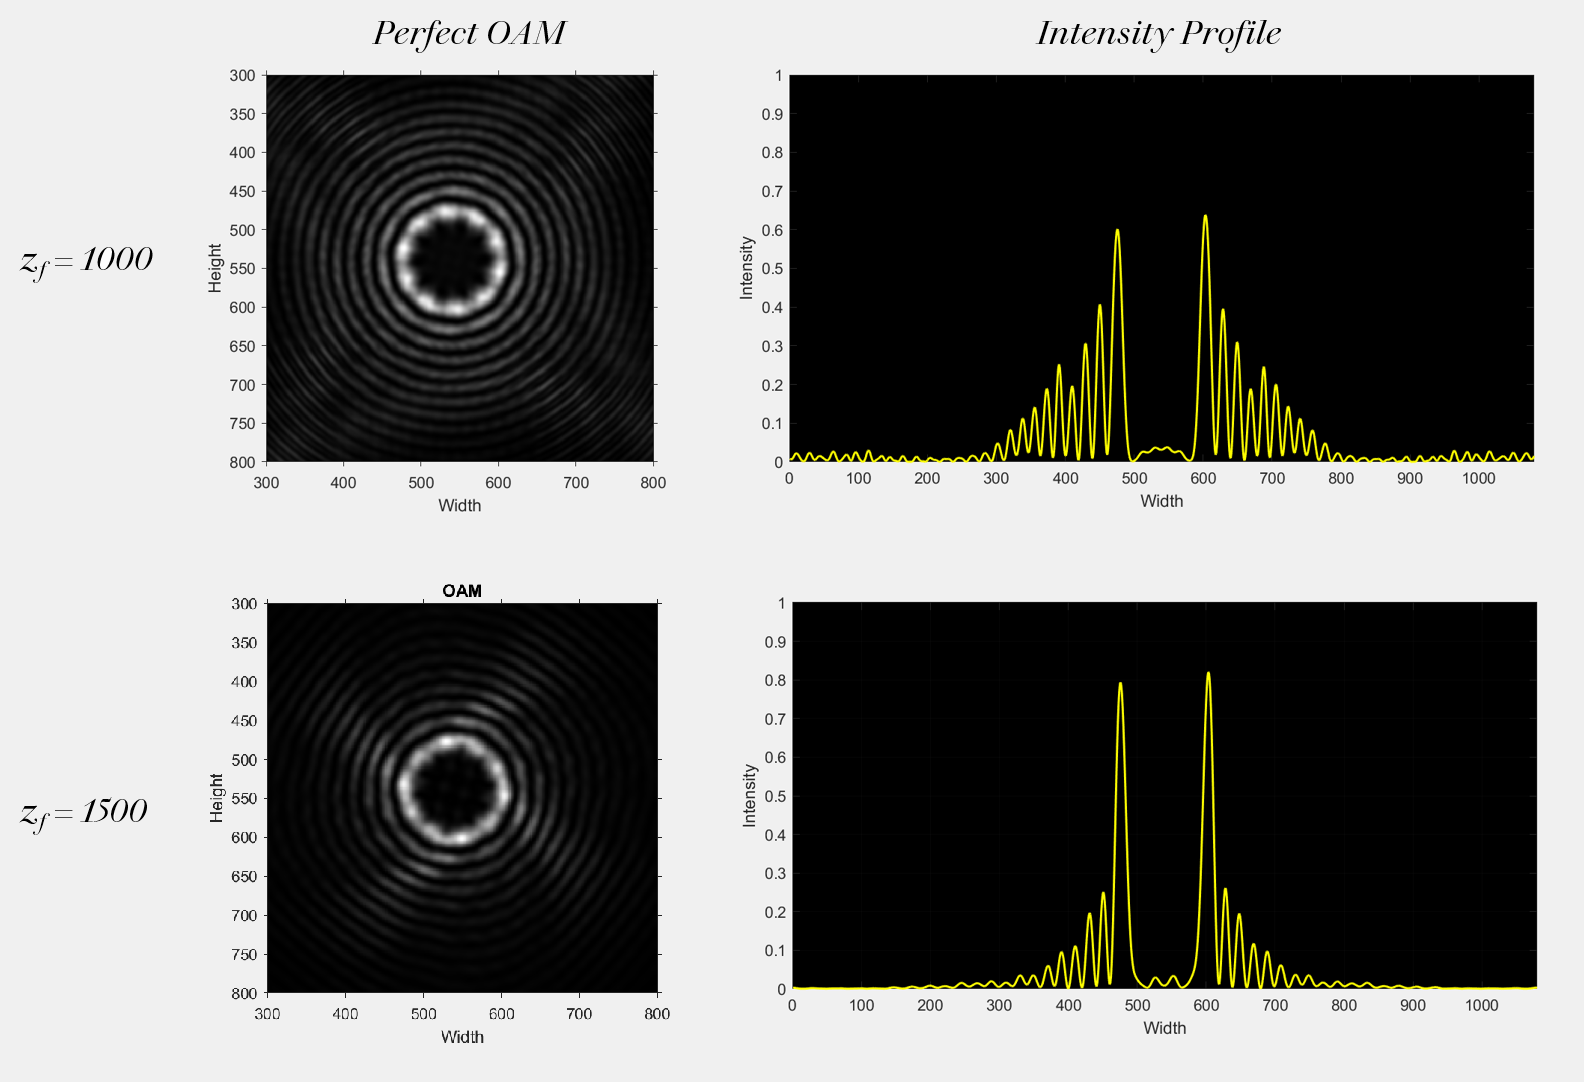
\includegraphics[width=14cm]{images/c04/Different_zf_same_obs.png}
    \caption{Direct comparison between the perfect vortices' intensity field and profile of figures (\ref{fig:Vortices_r=50_z=1000}) and (\ref{fig:Vortices_r=50_z=1500}).}
    \label{fig:perfects_1000_vs_1500}
\end{figure}

Propagations towards infinity appear to follow the same trend. At this distance, the propagation type is different, as it uses Franuhoffer's integral instead of Fresnel's one. This translates to a different looking, yet essentially similar, vortex: again, most of the intensity is cramped in the main ring and there is a dark circular region within this ring. For future reference, the unobstructed propagations are shown in figure (\ref{fig:Vortices_r=0_z=inf}).

\begin{figure}[htbp]
    \centering
    \begin{subfigure}[b]{0.45\textwidth}
        \centering
        \includegraphics[width=\textwidth]{images/c04/type=0_r=0_zi=0_zf=Inf.eps}
        \caption{Regular vortex.}
    \end{subfigure}
    \hfill
    \begin{subfigure}[b]{0.45\textwidth}
        \centering
        \includegraphics[width=\textwidth]{images/c04/type=1_r=0_zi=0_zf=Inf.eps}
        \caption{Perfect vortex.}
    \end{subfigure}
    \caption{Unobstructed vortices directly propagated through infinity.}
    \label{fig:Vortices_r=0_z=inf}
\end{figure}

Just as in the previous cases, when the obstruction size grows, the vortices deform progressively, with the perfect ones deforming significantly less in shape and time than regular ones. This progression is shown below in figures (\ref{fig:Vortices_r=20_z=inf}, \ref{fig:Vortices_r=40_z=inf}, \ref{fig:Vortices_r=60_z=inf} and \ref{fig:Vortices_r=100_z=inf}).

\begin{figure}[htbp]
    \centering
    \begin{subfigure}[b]{0.45\textwidth}
        \centering
        \includegraphics[width=\textwidth]{images/c04/type=0_r=0_zi=0_zf=Inf_TC.eps}
        \caption{Regular vortex.}
    \end{subfigure}
    \hfill
    \begin{subfigure}[b]{0.45\textwidth}
        \centering
        \includegraphics[width=\textwidth]{images/c04/type=1_r=0_zi=0_zf=Inf_TC.eps}
        \caption{Perfect vortex.}
    \end{subfigure}
    \caption{Topological charge of the unobstructed vortices propagated through infinity.}
    \label{fig:Vortices_r=0_z=inf_TC}
\end{figure}

%Examining the topological charges does bring to attention that the perfect vortex's phase mask is completely erratic, and does not seem to reflect its topological charge in this manner. On the other hand, regular vortices do keep their topological charge intact, at least apparently, at this distance and propagation type. This trend is consistent for all perfect vortices' propagations through $z_f = \infty$, regardless of obstruction radius.

\begin{figure}[htbp]
    \centering
    \begin{subfigure}[b]{0.45\textwidth}
        \centering
        \includegraphics[width=\textwidth]{images/c04/type=0_r=20_zi=0_zf=Inf.eps}
        \caption{Regular vortex.}
    \end{subfigure}
    \hfill
    \begin{subfigure}[b]{0.45\textwidth}
        \centering
        \includegraphics[width=\textwidth]{images/c04/type=1_r=20_zi=0_zf=Inf.eps}
        \caption{Perfect vortex.}
    \end{subfigure}
    \caption{Vortices directly propagated through infinity with a 20 [px] obstruction radius.}
    \label{fig:Vortices_r=20_z=inf}
\end{figure}

\begin{figure}[htbp]
    \centering
    \begin{subfigure}[b]{0.45\textwidth}
        \centering
        \includegraphics[width=\textwidth]{images/c04/type=0_r=40_zi=0_zf=Inf.eps}
        \caption{Regular vortex.}
    \end{subfigure}
    \hfill
    \begin{subfigure}[b]{0.45\textwidth}
        \centering
        \includegraphics[width=\textwidth]{images/c04/type=1_r=40_zi=0_zf=Inf.eps}
        \caption{Perfect vortex.}
    \end{subfigure}
    \caption{Vortices directly propagated through infinity with a 40 [px] obstruction radius.}
    \label{fig:Vortices_r=40_z=inf}
\end{figure}

\begin{figure}[htbp]
    \centering
    \begin{subfigure}[b]{0.45\textwidth}
        \centering
        \includegraphics[width=\textwidth]{images/c04/type=0_r=50_zi=0_zf=Inf.eps}
        \caption{Regular vortex.}
    \end{subfigure}
    \hfill
    \begin{subfigure}[b]{0.45\textwidth}
        \centering
        \includegraphics[width=\textwidth]{images/c04/type=1_r=50_zi=0_zf=Inf.eps}
        \caption{Perfect vortex.}
    \end{subfigure}
    \caption{Vortices directly propagated through infinity with a 50 [px] obstruction radius.}
    \label{fig:Vortices_r=60_z=inf}
\end{figure}

\begin{figure}[htbp]
    \centering
    \begin{subfigure}[b]{0.45\textwidth}
        \centering
        \includegraphics[width=\textwidth]{images/c04/type=0_r=100_zi=0_zf=Inf.eps}
        \caption{Regular vortex.}
    \end{subfigure}
    \hfill
    \begin{subfigure}[b]{0.45\textwidth}
        \centering
        \includegraphics[width=\textwidth]{images/c04/type=1_r=100_zi=0_zf=Inf.eps}
        \caption{Perfect vortex.}
    \end{subfigure}
    \caption{Vortices directly propagated through infinity with a 100 [px] obstruction radius.}
    \label{fig:Vortices_r=100_z=inf}
\end{figure}

Once again, the perfect vortex showed to be more resilient than the regular one. Interestingly, the perfect vortex does not change much, even less so than at shorter distances like 1000 and 1500 [mm]. The main ring's brightness remained almost static throughout the obstruction's growth; still, a barely noticeable dim ``dot'' appears at the very center sometime in-between obstruction radii of 60 and 100 [px]. Barely, because it is already hard to detect by visual inspection on a zoomed-in image of the OAM, effectively showing a 200x200 image instead of the full 1080x1080 one. On the other hand, the regular vortex did not experience the same fate. At an obstruction radius of 20 [px], the main ring has already lost its shape, resembling the petals of a flower; in addition, at 40 [px] the central region lights up significantly. Furthermore, at 60 [px], the regular vortex's intensity profile looks more like a Gaussian and less like a vortex. These observations reinforce the idea that perfect vortices are extraordinarily resistant to deformations caused by central obstructions, compared to the more used regular vortices.

In figure (\ref{fig:r=50_comparison}), we can directly compare regular and perfect vortices with a fixed obstruction radius of 50 [px] at different propagation distances, in [mm]. Here, it is even more evident that perfect vortices preserve their original shape better than regular ones. Howbeit, the near-field propagation distance restriction for perfect vortices is also noticeable, as the vortex is completely deformed at $z_f = 2000$ [mm]. Even so, the intensity profile is showing more resilience than the regular one, under the same circumstances. 

\begin{figure}[htbp]
    \centering
    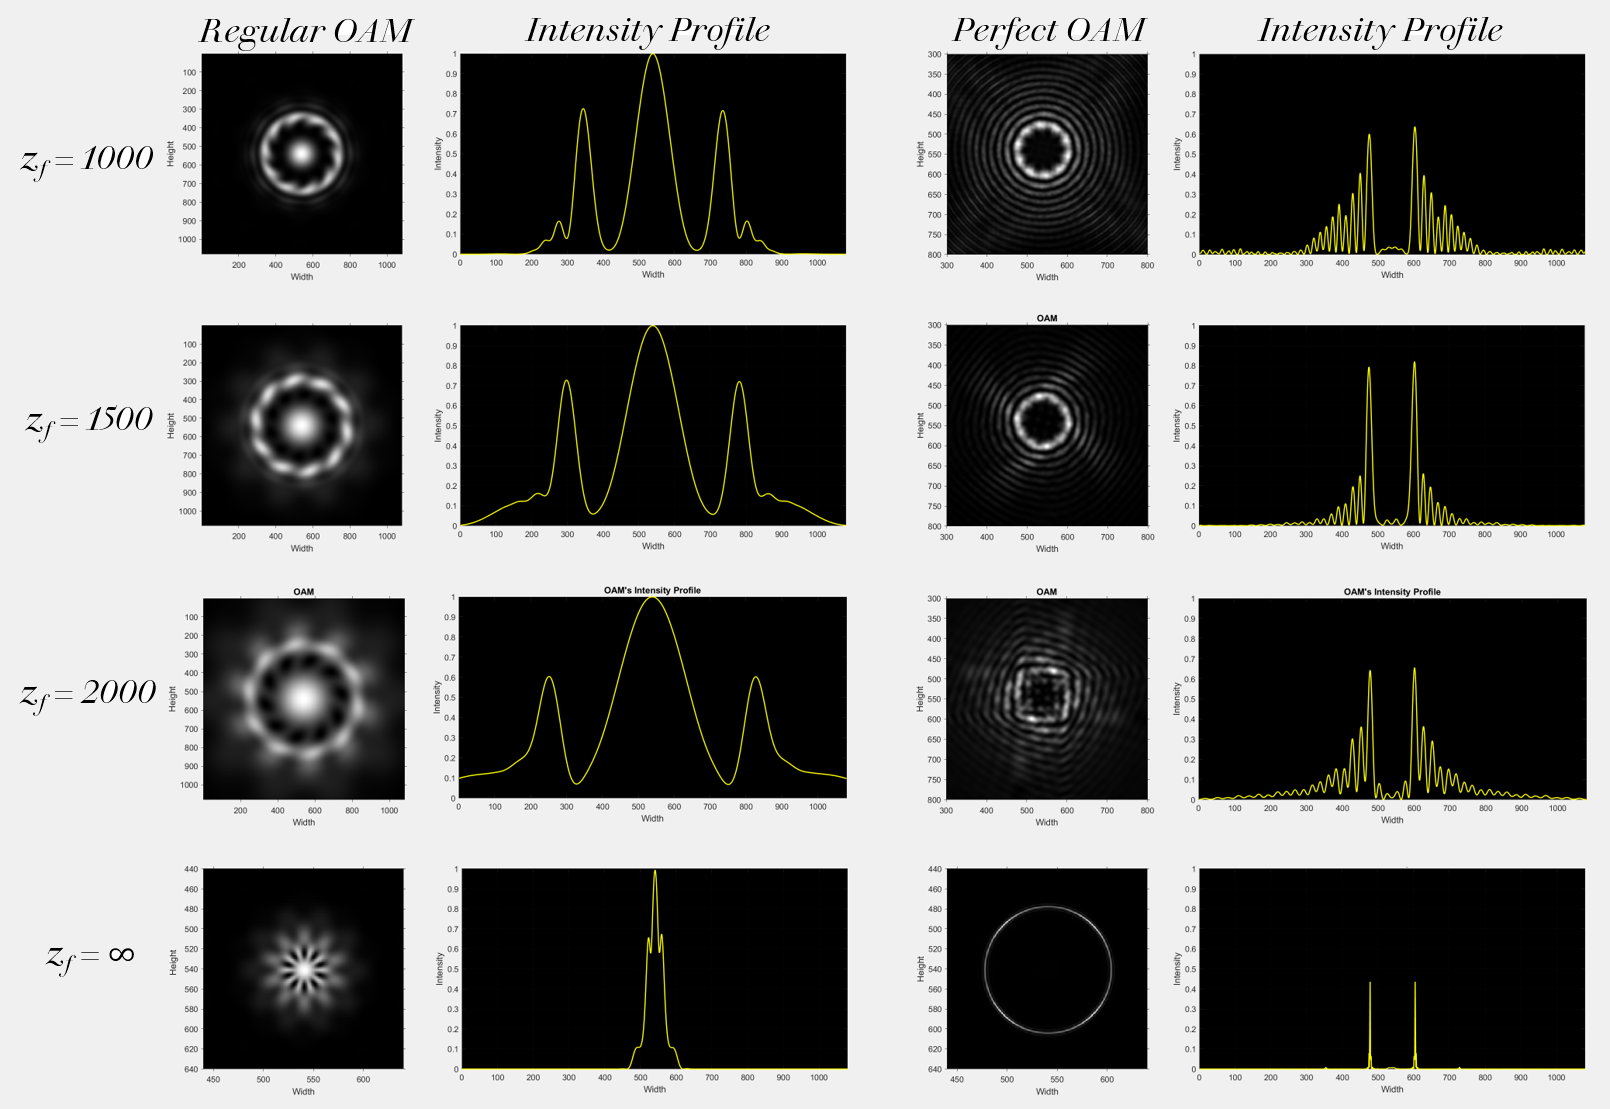
\includegraphics[width=\textwidth]{images/c04/r=50_distance_comparison.png}
    \caption{Comparison between different propagation distances with an obstruction radius of 50 [px].}
    \label{fig:r=50_comparison}
\end{figure}

\newpage
\section{Intensity Profiles Comparison}
This section presents directs comparisons between intensity profiles resulting from varying obstruction radius (in [px]) and propagation distance (in [mm]) among the same vortex type.

\begin{figure}[htbp]
    \centering
    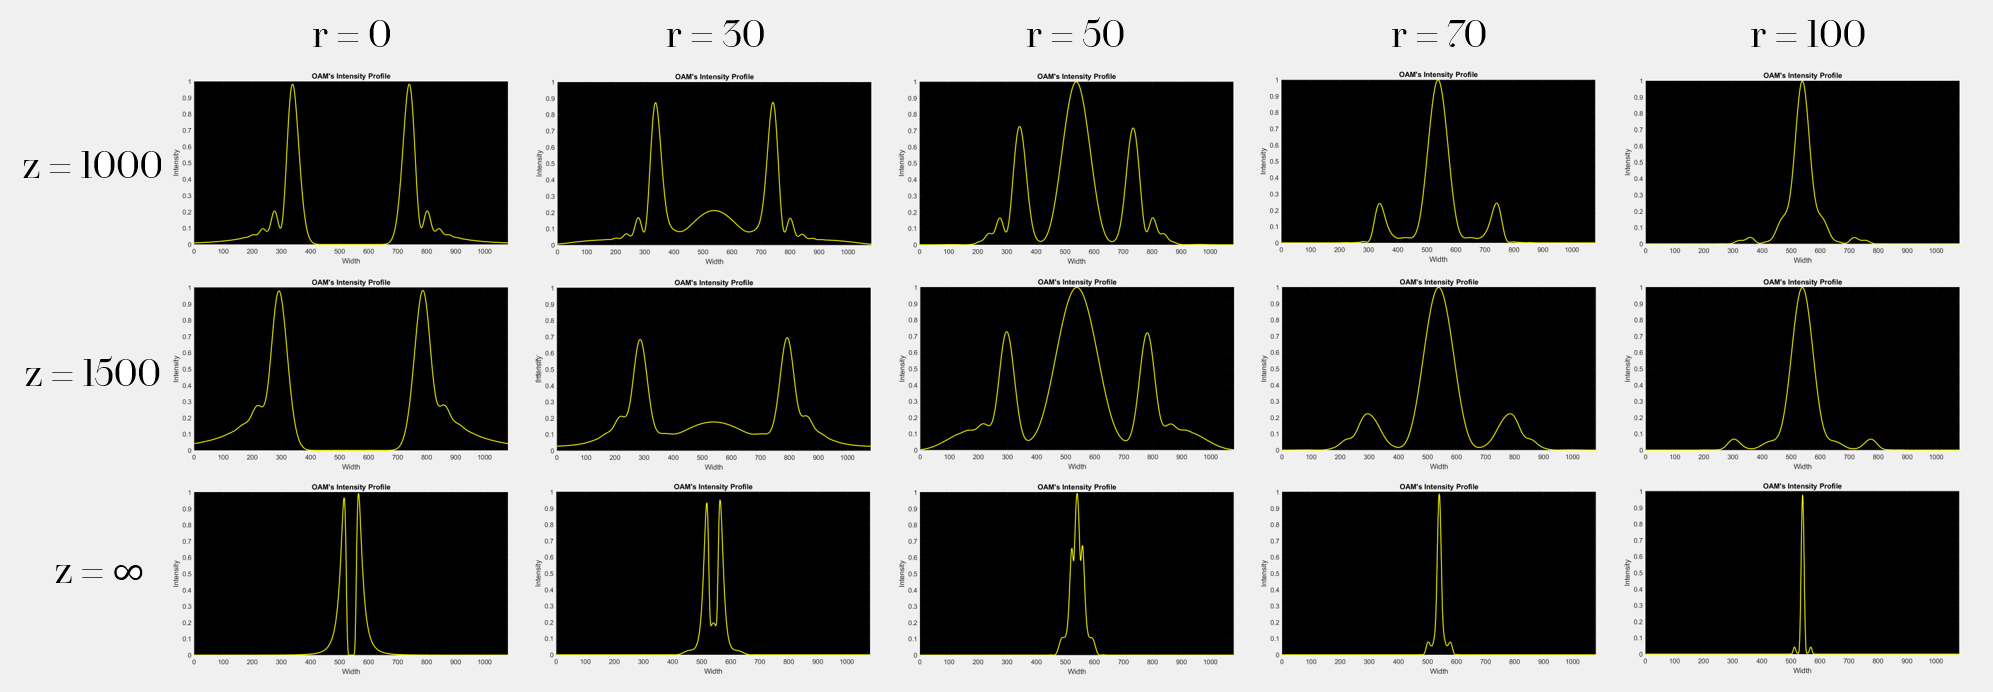
\includegraphics[width=15cm]{images/c04/Regular_Vortices-z_vs_r.png}
    \caption{Regular vortices' comparison from varying obstruction radius and propagation distance.}
    \label{fig:regular_r_vs_z}
\end{figure}

\begin{figure}[htbp]
    \centering
    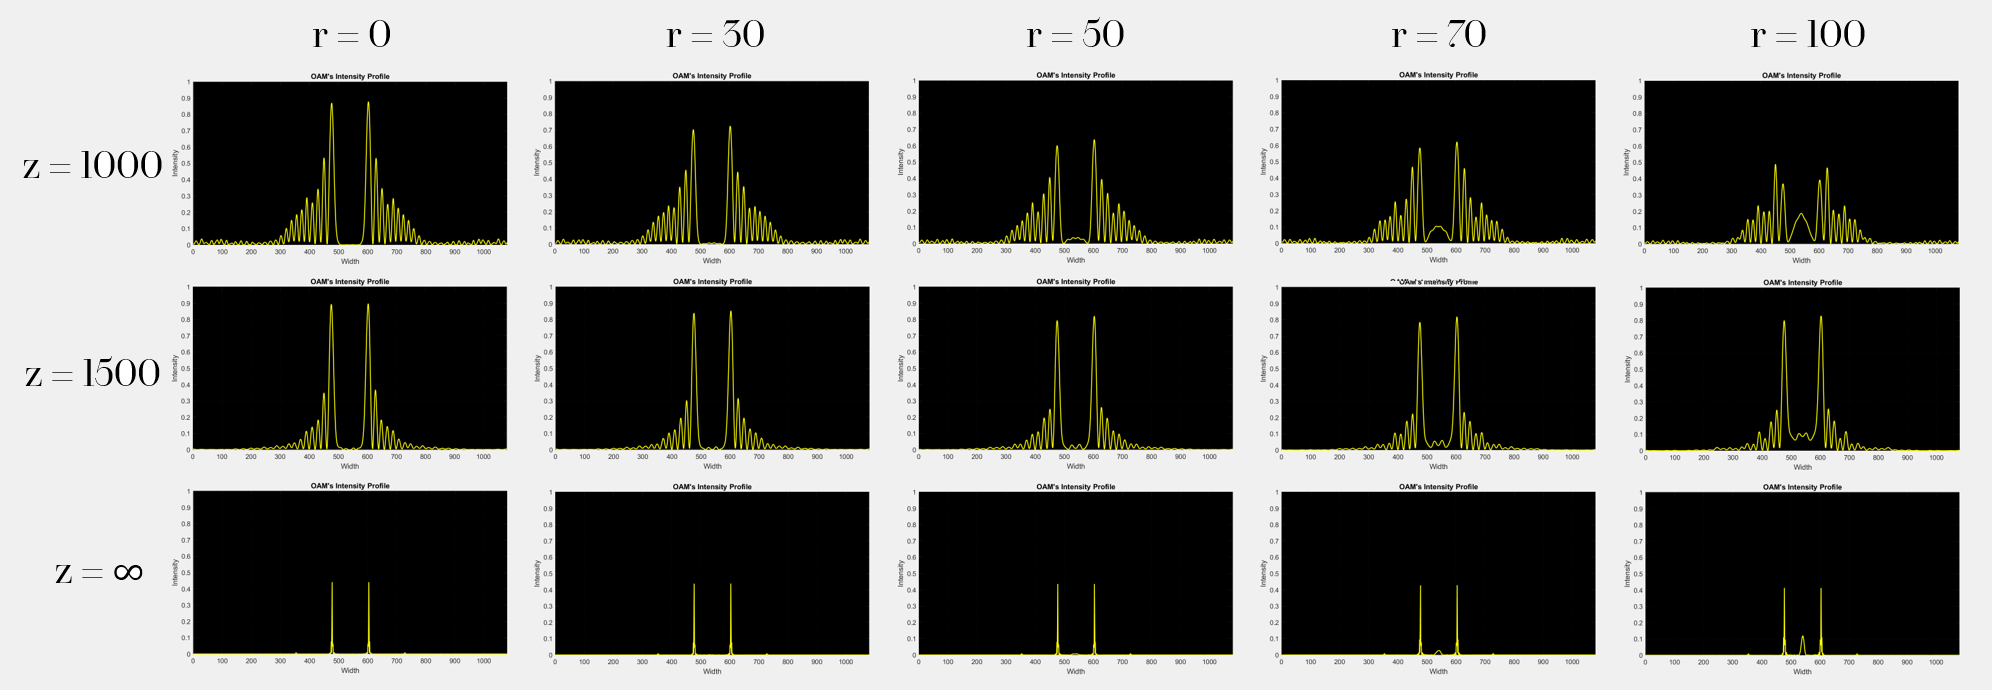
\includegraphics[width=15cm]{images/c04/Perfect_Vortices-z_vs_r.png}
    \caption{Perfect vortices' comparison from varying obstruction radius and propagation distance.}
    \label{fig:regular_r_vs_z}
\end{figure}


\newpage
\section{Regarding changes in other variables}
\label{c4:other arguments variations}

There is a myriad of variables involved in this simulation, and as expected, so are the possible outcomes of doing so. However, many of the latter are repetitive, sharing many similarities with the ones already presented in the previous sections. For instance, modifying fundamental variables such as state ($\ell$), $\sigma$, \textit{Rpx} and \textit{N} can certainly alter the vortices themselves, mostly changing their size, but also the number of rings surrounding the main ring.

Results of staged propagation were planned to be included, initially, to study propagations where the obstructions could have been located at arbitrary distances. However, they did not provide good results for the deformed it induced on the phase mask's edges. The propagation models (see section (\ref{c2:Near and Far Field Propagation}) and appendix (\ref{Scripts:Propagation}) for more information) induce errors caused by digital limitations like resolution and Fourier transform and integrals' approximations. These errors present themselves as deformation around the edges of the phase mask, and are cumulative as the same phase mask is re-propagated. To partially counter these effects, \textit{phase cleaning} should be applied. For the purposes of this work, and time limitations, it was not done; however, it is encouraged to do so to enhance the results that it can produce. 

For the previously stated reasons, unobstructed vortices propagated by stages produced worse-looking vortices than using direct propagation. For example, when propagating through a total distance $z_f$ of 1000 [mm], the vortices got worse when staged propagation took place by using $z_i$ distances like 100, 200 or 500 [mm].

Taking all of the above into consideration, it was determined that neither of these results belonged in this section as they do not provide new information regarding the vortices' resistance. In consequence, results obtained from varying these arguments will be shown in appendix (\ref{Complementary_Results}).

